\section{Теоретична част и постановка}
\label{sec:theory}
Целта на упражнението е изследване на корелационни зависимости и построяване на регресионни модели. При множествената линейна регресия се търси зависимост на променливата $z$ от независимите величини $w, x$ и $y$ във вида:
\begin{equation}
\label{eq:regression}
z = \beta_0 + w\beta_1 + x\beta_2 + y\beta_3
\end{equation}

Параметрите $\beta_i$ се намират чрез решаване на система от нормални линейни уравнения:
\begin{equation}
\label{eq:normal-system}
\begin{cases}
\beta_0 n + \beta_1 \sum w_i + \beta_2 \sum x_i + \beta_3 \sum y_i = \sum z_i \\
\beta_0 \sum w_i + \beta_1 \sum w_i^2 + \beta_2 \sum w_i x_i + \beta_3 \sum w_i y_i = \sum w_i z_i \\
\beta_0 \sum x_i + \beta_1 \sum w_i x_i + \beta_2 \sum x_i^2 + \beta_3 \sum x_i y_i = \sum x_i z_i \\
\beta_0 \sum y_i + \beta_1 \sum w_i y_i + \beta_2 \sum x_i y_i + \beta_3 \sum y_i^2 = \sum y_i z_i
\end{cases}
\end{equation}

\section{Задача 2: Решение на системата за Пример 3 (Таблица 3)}
\label{sec:table3}
Въз основа на данните от Таблица~3, системата е следната:
\begin{equation}
\label{eq:system3}
\begin{cases}
6\beta_0 + 4863\beta_1 + 8761\beta_2 + 654\beta_3 = 714 \\
4863\beta_0 + 4521899\beta_1 + 8519938\beta_2 + 620707\beta_3 = 667832 \\
8761\beta_0 + 8519938\beta_1 + 21022091\beta_2 + 905925\beta_3 = 1265493 \\
654\beta_0 + 620707\beta_1 + 905925\beta_2 + 137902\beta_3 = 100583
\end{cases}
\end{equation}

\subsection{Подробно решение чрез метода на Гаус}
За по-голяма прегледност работим с разширената матрица на системата:
\[
M = \left[ \begin{array}{cccc|c}
6 & 4863 & 8761 & 654 & 714 \\
4863 & 4521899 & 8519938 & 620707 & 667832 \\
8761 & 8519938 & 21022091 & 905925 & 1265493 \\
654 & 620707 & 905925 & 137902 & 100583
\end{array} \right]
\]

\textbf{Стъпка 1: Нормализиране на $R_1$ и елиминиране на $\beta_0$ от $R_2$, $R_3$, $R_4$.}

Разделяме $R_1$ на 6:
\[
R_1 \leftarrow \frac{R_1}{6} = [1,\; 810{,}5,\; 1460{,}1\overline{6},\; 109 \mid 119]
\]

След трансформациите $R_2 \leftarrow R_2 - 4863 R_1$,\; $R_3 \leftarrow R_3 - 8761 R_1$,\; $R_4 \leftarrow R_4 - 654 R_1$ матрицата придобива вида:
\[
\left[\begin{array}{cccc|c}
1      & 810{,}5     & 1460{,}17  & 109       & 119      \\
0      & 580437{,}5  & 1421667{,}5 & 90640     & 89135    \\
0      & 1420407{,}5 & 8229570{,}8 & -49324    & 222934   \\
0      & 90640       & -48424      & 66616     & 22757
\end{array}\right]
\]

\textbf{Стъпка 2: Нормализиране на $R_2$ и елиминиране на $\beta_1$ от $R_3$, $R_4$.}

Разделяме $R_2$ на $580437{,}5$:
\[
R_2 \leftarrow \frac{R_2}{580437{,}5} = [0,\; 1,\; 2{,}4493,\; 0{,}1562 \mid 0{,}1536]
\]

След $R_3 \leftarrow R_3 - 1420407{,}5\, R_2$ и $R_4 \leftarrow R_4 - 90640\, R_2$:
\[
\left[\begin{array}{cccc|c}
1 & 810{,}5 & 1460{,}17  & 109       & 119      \\
0 & 1       & 2{,}4493    & 0{,}1562  & 0{,}1536 \\
0 & 0       & 4750743{,}1 & -271120{,}7 & 4848{,}2 \\
0 & 0       & -270409{,}4 & 52461{,}5 & 8837{,}7
\end{array}\right]
\]

\textbf{Стъпка 3: Нормализиране на $R_3$ и елиминиране на $\beta_2$ от $R_4$.}

Разделяме $R_3$ на $4750743{,}1$:
\[
R_3 \leftarrow \frac{R_3}{4750743{,}1} = [0,\; 0,\; 1,\; -0{,}05707 \mid 0{,}001021]
\]

След $R_4 \leftarrow R_4 - (-270409{,}4)\, R_3$:
\[
\left[\begin{array}{cccc|c}
1 & 810{,}5 & 1460{,}17 & 109        & 119      \\
0 & 1       & 2{,}4493   & 0{,}1562   & 0{,}1536 \\
0 & 0       & 1          & -0{,}05707 & 0{,}001021 \\
0 & 0       & 0          & 37028{,}4  & 9113{,}3
\end{array}\right]
\]

\textbf{Стъпка 4: Обратна замяна.}

От $R_4$:
\[
\beta_3 = \frac{9113{,}3}{37028{,}4} \approx 0{,}2461
\]

От $R_3$: $\beta_2 = 0{,}001021 - (-0{,}05707)\cdot 0{,}2461 \approx 0{,}001021 + 0{,}014044 \approx 0{,}0150$

От $R_2$: $\beta_1 = 0{,}1536 - 2{,}4493\cdot 0{,}0150 - 0{,}1562\cdot 0{,}2461 \approx 0{,}1536 - 0{,}03674 - 0{,}03843 \approx 0{,}0784$

От $R_1$: $\beta_0 = 119 - 810{,}5\cdot 0{,}0784 - 1460{,}17\cdot 0{,}0150 - 109\cdot 0{,}2461 \approx 119 - 63{,}54 - 21{,}90 - 26{,}82 \approx 6{,}7013$

Получените параметри:
\begin{align*}
\beta_3 &= 0{,}2461 \\
\beta_2 &= 0{,}0150 \\
\beta_1 &= 0{,}0784 \\
\beta_0 &= 6{,}7013
\end{align*}

Получените стойности съвпадат с очакваните в условието (вж. Таблица~\ref{tab:results}).

\section{Задача 3: Пресмятане на регресия за Таблица 5}
\label{sec:table5}
Използваме данните от Таблица~5. Изчислените суми са:
\begin{itemize}
    \item $n = 6$
    \item $\sum w = 1670$, $\sum x = 355$, $\sum y = 149$, $\sum z = 138{,}1$
    \item $\sum w^2 = 641720$, $\sum x^2 = 46343$, $\sum y^2 = 10557$
    \item $\sum wx = 114071$, $\sum wy = 35495$, $\sum xy = 20819$
    \item $\sum wz = 49225{,}1$, $\sum xz = 11202{,}0$, $\sum yz = 4179{,}4$
\end{itemize}

Разширената матрица на системата е:
\begin{equation}
\label{eq:system5}
\left[\begin{array}{cccc|c}
6    & 1670   & 355    & 149   & 138{,}1   \\
1670 & 641720 & 114071 & 35495 & 49225{,}1 \\
355  & 114071 & 46343  & 20819 & 11202{,}0 \\
149  & 35495  & 20819  & 10557 & 4179{,}4
\end{array}\right]
\end{equation}

\subsection{Подробно решение чрез метода на Гаус}

\textbf{Стъпка 1: Нормализиране на $R_1$ и елиминиране на $\beta_0$ от $R_2$, $R_3$, $R_4$.}

Разделяме $R_1$ на 6:
\[
R_1 \leftarrow \frac{R_1}{6} = [1,\; 278{,}3\overline{3},\; 59{,}1\overline{6},\; 24{,}8\overline{3} \mid 23{,}01\overline{6}]
\]

След $R_2 \leftarrow R_2 - 1670\,R_1$,\; $R_3 \leftarrow R_3 - 355\,R_1$,\; $R_4 \leftarrow R_4 - 149\,R_1$:
\[
\left[\begin{array}{cccc|c}
1 & 278{,}33 & 59{,}17 & 24{,}83 & 23{,}02 \\
0 & 176903{,}3 & 15262{,}6 & -5976{,}7 & 10787{,}2 \\
0 & 15262{,}7 & 25338{,}8 & 12003{,}2 & 3031{,}0 \\
0 & -5976{,}7 & 12003{,}2 & 6856{,}8 & 749{,}9
\end{array}\right]
\]

\textbf{Стъпка 2: Нормализиране на $R_2$ и елиминиране на $\beta_1$ от $R_3$, $R_4$.}

Разделяме $R_2$ на $176903{,}3$:
\[
R_2 \leftarrow \frac{R_2}{176903{,}3} = [0,\; 1,\; 0{,}08627,\; -0{,}03379 \mid 0{,}06098]
\]

След $R_3 \leftarrow R_3 - 15262{,}7\,R_2$ и $R_4 \leftarrow R_4 - (-5976{,}7)\,R_2$:
\[
\left[\begin{array}{cccc|c}
1 & 278{,}33 & 59{,}17 & 24{,}83 & 23{,}02 \\
0 & 1 & 0{,}08627 & -0{,}03379 & 0{,}06098 \\
0 & 0 & 24022{,}2 & 12518{,}9 & 2100{,}5 \\
0 & 0 & 12518{,}8 & 6654{,}9 & 1114{,}3
\end{array}\right]
\]

\textbf{Стъпка 3: Нормализиране на $R_3$ и елиминиране на $\beta_2$ от $R_4$.}

Разделяме $R_3$ на $24022{,}2$:
\[
R_3 \leftarrow \frac{R_3}{24022{,}2} = [0,\; 0,\; 1,\; 0{,}52114 \mid 0{,}08744]
\]

След $R_4 \leftarrow R_4 - 12518{,}8\,R_3$:
\[
\left[\begin{array}{cccc|c}
1 & 278{,}33 & 59{,}17 & 24{,}83 & 23{,}02 \\
0 & 1 & 0{,}08627 & -0{,}03379 & 0{,}06098 \\
0 & 0 & 1 & 0{,}52114 & 0{,}08744 \\
0 & 0 & 0 & 130{,}9 & 19{,}6
\end{array}\right]
\]

\textbf{Стъпка 4: Обратна замяна.}

От $R_4$:
\[
\beta_3 = \frac{19{,}6}{130{,}9} \approx 0{,}1510
\]

От $R_3$: $\beta_2 = 0{,}08744 - 0{,}52114\cdot 0{,}1510 \approx 0{,}08744 - 0{,}07869 \approx 0{,}0087$

От $R_2$: $\beta_1 = 0{,}06098 - 0{,}08627\cdot 0{,}0087 - (-0{,}03379)\cdot 0{,}1510 \approx 0{,}06098 - 0{,}00075 + 0{,}00510 \approx 0{,}0653$

От $R_1$: $\beta_0 = 23{,}02 - 278{,}33\cdot 0{,}0653 - 59{,}17\cdot 0{,}0087 - 24{,}83\cdot 0{,}1510 \approx 23{,}02 - 18{,}17 - 0{,}52 - 3{,}75 \approx 0{,}5665$

Получените параметри:
\begin{align*}
\beta_3 &= 0{,}1510 \\
\beta_2 &= 0{,}0087 \\
\beta_1 &= 0{,}0653 \\
\beta_0 &= 0{,}5665
\end{align*}

\section{Задача 4: Отчет (Table 4)}
\label{sec:report}
\begin{table}[h]
\centering
\caption{Сравнителен отчет на получените резултати}
\label{tab:results}
\begin{tabular}{llcc}
\toprule
\textbf{Тест} & \textbf{Параметър} & \textbf{Очаквана стойност} & \textbf{Действителна стойност} \\ \midrule
Таблица 3 & $\beta_0$ & 6,7013 & 6,7013 \\
          & $\beta_1$ & 0,0784 & 0,0784 \\
          & $\beta_2$ & 0,0150 & 0,0150 \\
          & $\beta_3$ & 0,2461 & 0,2461 \\\bottomrule
\end{tabular}
\end{table}
\begin{figure}[h!]
\centering
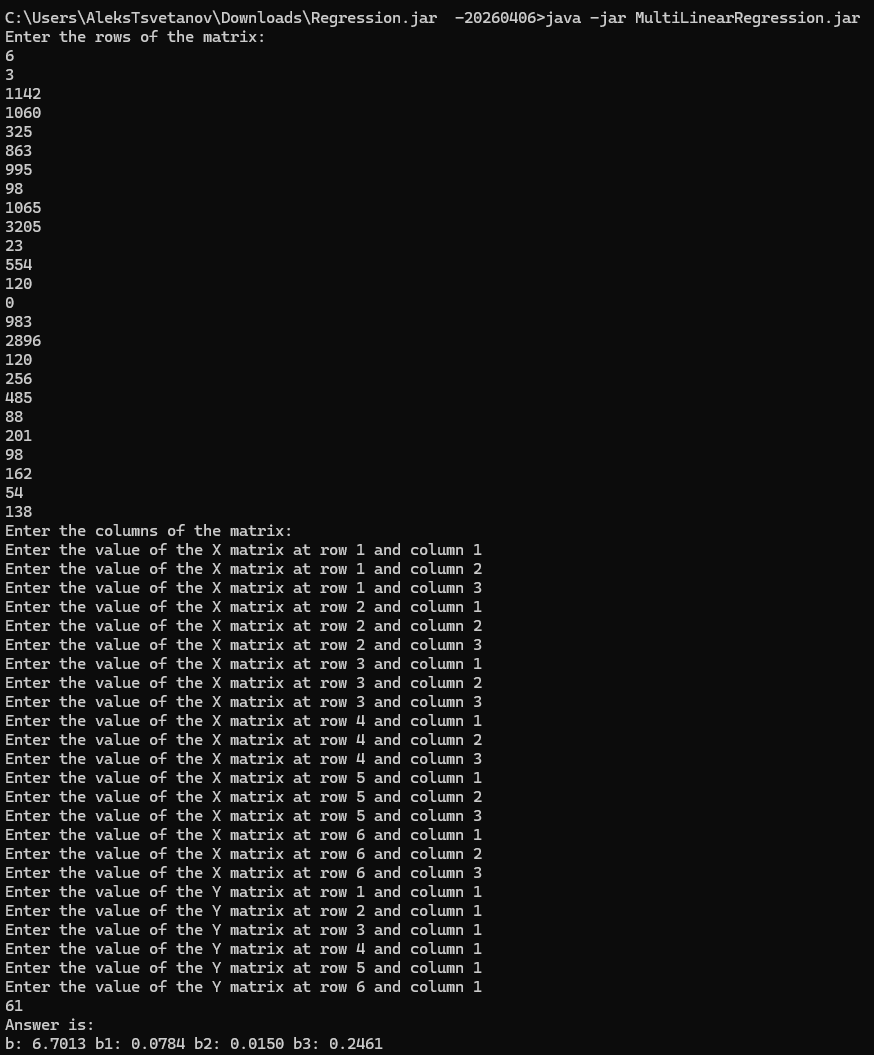
\includegraphics[width=0.75\textwidth, trim=0 0 0 20pt, clip]{images/regression run.png}
\caption{Резултати от регресионния анализ}
\label{fig:regression}
\end{figure}

\section{Визуализация на данни и допълнителни ресурси}
В съответствие със задачите беше разучена работата с \textbf{Excel Analysis ToolPak} за генериране на случайни числа, създаване на честотни разпределения и визуализация чрез хистограми, диаграми на разсейване (scatter plots) и линейни графики. Видео ресурсът на Khan Academy демонстрира практическото приложение на линейните модели за интерполация (оценка между точки) и екстраполация (прогнозиране извън наличните данни).